\documentclass[12pt,a4paper]{article}
\usepackage[utf8]{inputenc}
\usepackage[T1]{fontenc}
\usepackage[serbian]{babel}
\usepackage{amsmath, amssymb}
\usepackage{graphicx}
\usepackage{booktabs}
\usepackage{array}
\usepackage{multirow}
\usepackage{tikz}
\usetikzlibrary{positioning, arrows.meta}
\usepackage{float}
\usepackage{caption}
\usepackage{geometry}
\usepackage{hyperref}
\geometry{margin=2.5cm}
\graphicspath{{src/homework_2/}}

\begin{document}

% ── Naslovna strana ───────────────────────────────────────────────────────────
\begin{titlepage}
  \centering
  \vspace*{1.5cm}
  
\includegraphics[width=0.32\textwidth]{etf_logo.png}\\[1.8cm]
  {\large Univerzitet u Beogradu}\\[0.3em]
  {\large Elektrotehnički fakultet}\\[2.5cm]
  {\LARGE\textbf{Drugi domaći zadatak}}\\[0.8em]
  {\Large Zaključivanje u (dinamičkim) Bayesovim mrežama}\\[0.6em]
  {\large Predmet: Veštačka inteligencija (13E054VI)}\\[3.5cm]
  {\large Mihajlo Stevanović}\\[0.3em]
  {\large 2022/0315}\\[2cm]
  {\large Beograd, \the\year}
\end{titlepage}

% ─────────────────────────────────────────────────────────────────────────────
\section{Zadatak 1}

\subsection{Uvod}

Dat je skup tabela uslovnih verovatnoća (TUV) koji jednoznačno određuje jednu Bayesovu mrežu:

\begin{center}
\begin{tabular}{c|c}
  $A$ & $P(b^- \mid A)$ \\ \hline
  $a^-$ & 0.3 \\
  $a^+$ & 0.8 \\
\end{tabular}
\quad
\begin{tabular}{c|c}
  $A$ & $P(c^- \mid A)$ \\ \hline
  $a^-$ & 0.4 \\
  $a^+$ & 0.6 \\
\end{tabular}
\quad
\begin{tabular}{c|c}
  $D$ & $P(f^- \mid D)$ \\ \hline
  $d^-$ & 0.2 \\
  $d^+$ & 0.6 \\
\end{tabular}
\end{center}

\vspace{0.5em}

\begin{center}
\begin{tabular}{cc|c}
  $A$ & $B$ & $P(d^- \mid A, B)$ \\ \hline
  $a^-$ & $b^-$ & 0.1 \\
  $a^-$ & $b^+$ & 0.5 \\
  $a^+$ & $b^-$ & 0.2 \\
  $a^+$ & $b^+$ & 0.8 \\
\end{tabular}
\qquad
\begin{tabular}{cc|c}
  $C$ & $D$ & $P(e^- \mid C, D)$ \\ \hline
  $c^-$ & $d^-$ & 0.3 \\
  $c^-$ & $d^+$ & 0.8 \\
  $c^+$ & $d^-$ & 0.6 \\
  $c^+$ & $d^+$ & 0.6 \\
\end{tabular}
\end{center}

\vspace{0.3em}
\begin{center}
  $P(a^-) = 0.3$
\end{center}

Na osnovu datih TUV potrebno je konstruisati odgovarajući usmereni aciklični graf (UAG).
Zatim treba proceniti uslovnu verovatnoću $P(b^+\mid e^-,f^-)$ korišćenjem tri pristupa:
egzaktnom metodom eliminacije promenljivih, aproksimativnim uzorkovanjem sa odbacivanjem
i Gibsovim uzorkovanjem.

Za Monte Carlo metode treba odrediti veličinu uzorka $N$ takvu da standardne devijacije obe
metode budu otprilike jednake, a zatim sprovesti $N_r = 100$ nezavisnih ponovljanja i prikazati
histograme procena, uz naznačene vrednosti srednje vrednosti, standardne devijacije i tačnog
rezultata.

% ─────────────────────────────────────────────────────────────────────────────
\subsection{Rezultati}

\subsubsection*{Usmereni aciklični graf}

Svaka TUV opisuje zavisnost jedne promenljive od njenih roditelja, pa se grane grafa
direktno čitaju iz argumenta uslovne verovatnoće. Promenljiva $A$ nema roditelja i
predstavlja koren. Od nje direktno zavise $B$, $C$ i $D$; promenljiva $D$ ima još jednog
roditelja - $B$. Čvor $E$ zavisi od para $(C, D)$, a $F$ isključivo od $D$.

Združena raspodela svih šest promenljivih faktorizuje se kao:
\[
  P(A,B,C,D,E,F) = P(A)\cdot P(B\mid A)\cdot P(C\mid A)\cdot P(D\mid A,B)
                   \cdot P(E\mid C,D)\cdot P(F\mid D).
\]

Iz ove faktorizacije slede i relacije uslovne nezavisnosti: uz poznato $A$, promenljive
$B$ i $C$ postaju uslovno nezavisne; uz poznato $D$, promenljiva $F$ postaje nezavisna od
svih ostalih; uz poznate $C$ i $D$, promenljiva $E$ ne zavisi od $\{A, B, F\}$.
Konstruisani graf prikazan je na slici~\ref{fig:dag}.

\begin{figure}[H]
  \centering
  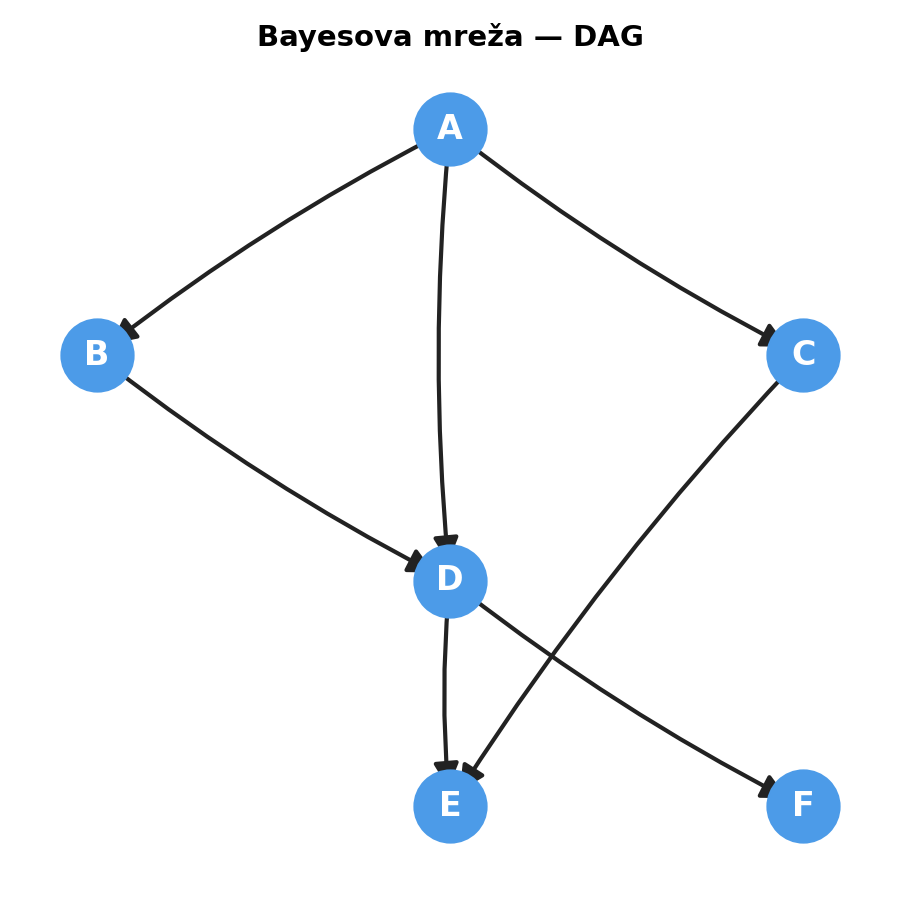
\includegraphics[width=0.45\textwidth]{dag.png}
  \caption{Usmereni aciklični graf Bayesove mreže.}
  \label{fig:dag}
\end{figure}

% ── VE ───────────────────────────────────────────────────────────────────────
\subsubsection*{Metoda eliminacije promenljivih}

Tražena veličina je $P(b^+\mid e^-,f^-) = P(b^+, e^-, f^-)\,/\,P(e^-, f^-)$.
Uvođenjem indikatora dokaza $\phi_E(C,D) = P(e^-\mid C,D)$ i $\phi_F(D) = P(f^-\mid D)$,
nenormalizovana raspodela po $B$ zapisuje se kao:
\[
  P(B, e^-, f^-) = \sum_A\sum_C\sum_D
    P(A)\cdot P(B\mid A)\cdot P(C\mid A)\cdot P(D\mid A,B)
    \cdot \phi_E(C,D)\cdot \phi_F(D).
\]

Skrivene promenljive $\{C, A, D\}$ eliminišemo tim redom. Redosled nije proizvoljan -
bira se tako da međufaktori ostanu što manjeg domena.
$C$ se eliminiše prva jer učestvuje samo u dva faktora ($P(C\mid A)$ i $\phi_E$);
njihovim množenjem i sumiranjem nastaje $h_1(A,D)$ - faktor samo dve promenljive.
Da smo počeli od $A$, koji se pojavljuje u četiri faktora, odmah bi nastao faktor
nad $(B,C,D)$ - tabela osam vrednosti i znatno skuplja operacija.

Nakon eliminacije $C$ preostaje: $P(A)$, $P(B\mid A)$, $P(D\mid A,B)$, $h_1(A,D)$, $\phi_F(D)$.
U ovoj tački redosled $A \to D$ i $D \to A$ su podjednako složeni: u oba slučaja
nastaje međuproizvod nad $(A,B,D)$ i rezultujući faktor dve promenljive.
Odabran je redosled $A \to D$.

\paragraph{Korak 1 - eliminacija $C$.}
Množimo $P(C\mid A)$ i $\phi_E(C,D)$, pa sumiramo po $C$:
\[
  h_1(A,D) = \sum_C P(C\mid A)\cdot P(e^-\mid C,D).
\]

\begin{center}
\begin{tabular}{cc|cc|c}
  \toprule
  $A$ & $D$ & doprinos $c^-$ & doprinos $c^+$ & $h_1(A,D)$ \\
  \midrule
  $a^-$ & $d^-$ & $0.4\cdot 0.3 = 0.120$ & $0.6\cdot 0.6 = 0.360$ & $0.48$ \\
  $a^-$ & $d^+$ & $0.4\cdot 0.8 = 0.320$ & $0.6\cdot 0.6 = 0.360$ & $0.68$ \\
  $a^+$ & $d^-$ & $0.6\cdot 0.3 = 0.180$ & $0.4\cdot 0.6 = 0.240$ & $0.42$ \\
  $a^+$ & $d^+$ & $0.6\cdot 0.8 = 0.480$ & $0.4\cdot 0.6 = 0.240$ & $0.72$ \\
  \bottomrule
\end{tabular}
\end{center}

\paragraph{Korak 2 - eliminacija $A$.}
Preostali faktori koji sadrže $A$ su $P(A)$, $P(B\mid A)$, $P(D\mid A,B)$ i $h_1(A,D)$:
\[
  h_2(B,D) = \sum_A P(A)\cdot P(B\mid A)\cdot P(D\mid A,B)\cdot h_1(A,D).
\]

\begin{center}
\begin{tabular}{cc|c}
  \toprule
  $B$ & $D$ & $h_2(B,D)$ \\
  \midrule
  $b^-$ & $d^-$ & $0.3\!\cdot\!0.3\!\cdot\!0.1\!\cdot\!0.48 + 0.7\!\cdot\!0.8\!\cdot\!0.2\!\cdot\!0.42
                   = 0.00432 + 0.04704 = 0.05136$ \\
  $b^-$ & $d^+$ & $0.3\!\cdot\!0.3\!\cdot\!0.9\!\cdot\!0.68 + 0.7\!\cdot\!0.8\!\cdot\!0.8\!\cdot\!0.72
                   = 0.05508 + 0.32256 = 0.37764$ \\
  $b^+$ & $d^-$ & $0.3\!\cdot\!0.7\!\cdot\!0.5\!\cdot\!0.48 + 0.7\!\cdot\!0.2\!\cdot\!0.8\!\cdot\!0.42
                   = 0.05040 + 0.04704 = 0.09744$ \\
  $b^+$ & $d^+$ & $0.3\!\cdot\!0.7\!\cdot\!0.5\!\cdot\!0.68 + 0.7\!\cdot\!0.2\!\cdot\!0.2\!\cdot\!0.72
                   = 0.07140 + 0.02016 = 0.09156$ \\
  \bottomrule
\end{tabular}
\end{center}

\paragraph{Korak 3 - eliminacija $D$.}
Na kraju množimo $h_2(B,D)$ i $\phi_F(D) = P(f^-\mid D)$, pa sumiramo po $D$:
\[
  h_3(B) = \sum_D h_2(B,D)\cdot P(f^-\mid D).
\]

\begin{center}
\begin{tabular}{c|l|c}
  \toprule
  $B$ & Razvoj & $h_3(B)$ \\
  \midrule
  $b^-$ & $0.05136\cdot 0.2 + 0.37764\cdot 0.6$ & $0.236856$ \\
  $b^+$ & $0.09744\cdot 0.2 + 0.09156\cdot 0.6$ & $0.074424$ \\
  \bottomrule
\end{tabular}
\end{center}

Zbir ovih vrednosti daje normalizacioni faktor, koji je ujedno i stopa prihvatanja za
uzorkovanje sa odbacivanjem:
\[
  P(e^-,f^-) = 0.236856 + 0.074424 = 0.311280.
\]

Normalizacijom dobijamo tačan rezultat:
\[
  \boxed{P(b^+\mid e^-,f^-) = \frac{0.074424}{0.311280} \approx 0.2391.}
\]

% ── Rejection Sampling ────────────────────────────────────────────────────────
\subsubsection*{Uzorkovanje sa odbacivanjem}

Svaki uzorak se generiše topološkim obilaskom grafa iz apriori raspodela:
\[
  A \sim P(A),\quad B \sim P(B\mid A),\quad C \sim P(C\mid A),\quad
  D \sim P(D\mid A,B),\quad E \sim P(E\mid C,D),\quad F \sim P(F\mid D).
\]
Uzorak se zadržava jedino ako važi $E = e^-$ i $F = f^-$;
u suprotnom se odbacuje i proces se ponavlja.
Estimator se formira kao relativna frekvencija vrednosti $B = b^+$ među prihvaćenim uzorcima:
\[
  \hat{P}(b^+\mid e^-,f^-) = \frac{\#\{i : B_i = b^+\}}{N_{\mathrm{prihv.}}}.
\]

Budući da je $P(e^-,f^-) = 0.3113$, otprilike svaki treći generisani uzorak biva prihvaćen.
Ovo je ključna mana metode: u slučaju retkih dokaza stopa prihvatanja eksponencijalno opada
sa brojem dokaznih promenljivih, pa je potrebno generisati znatno više uzoraka nego što
se na kraju koristi.

Veličinu uzorka $N_\mathrm{RS}$ biramo tako da standardna devijacija estimatora bude
$\sigma_0 = 0.025$. Kako estimator ima Bernulijevu varijansu podeljenu efektivnim
brojem prihvaćenih uzoraka:
\[
  \sigma_\mathrm{RS} = \sqrt{\frac{p(1-p)}{P(e^-,f^-)\cdot N_\mathrm{RS}}},
\]
gde $p \approx 0.2391$, rešavanjem po $N_\mathrm{RS}$ dobijamo:
\[
  N_\mathrm{RS} = \left\lceil \frac{p(1-p)}{P(e^-,f^-)\cdot\sigma_0^2} \right\rceil
  = \left\lceil \frac{0.2391\cdot 0.7609}{0.311280\cdot 0.000625} \right\rceil = 936.
\]
Od 936 generisanih uzoraka, prosečno se prihvata $936\cdot 0.3113 \approx 291$.

% ── Gibbs ────────────────────────────────────────────────────────────────────
\subsubsection*{Gibsovo uzorkovanje}

Za razliku od uzorkovanja sa odbacivanjem, Gibsovo uzorkovanje ne generiše uzorke iz
apriorne raspodele već konstruiše Markovljev lanac čija je stacionarna raspodela upravo
aposteriorna raspodela $P(A,B,C,D\mid e^-,f^-)$. U svakom koraku, jedna promenljiva
se uzorkuje iz njene uslovne raspodele uz fiksirane vrednosti svih ostalih i fiksirane
evidencije $E=e^-$, $F=f^-$.

Uslovne raspodele (Markovljev blanket svake promenljive) su:
\begin{align*}
  P(A \mid B,C,D,e^-,f^-) &\propto P(A)\cdot P(B\mid A)\cdot P(C\mid A)\cdot P(D\mid A,B),\\
  P(B \mid A,D,e^-,f^-)   &\propto P(B\mid A)\cdot P(D\mid A,B),\\
  P(C \mid A,D,e^-,f^-)   &\propto P(C\mid A)\cdot P(e^-\mid C,D),\\
  P(D \mid A,B,C,e^-,f^-) &\propto P(D\mid A,B)\cdot P(e^-\mid C,D)\cdot P(f^-\mid D).
\end{align*}
Svaki izraz na desnoj strani je nenormalizovan; normalizacija se vrši deljenjem sa zbirom
vrednosti za obe moguće vrednosti odgovarajuće promenljive.

Uzorkovanje kreće od nasumične inicijalizacije i ciklično obilazi promenljive redom $A, B, C, D$.
Prvih $N_\mathrm{burn} = 200$ odbiraka odbacujemo, jer lanac u toj fazi još konvergira ka
stacionarnoj raspodeli i odbirci su zavisni od početnih vrednosti. Tek nakon toga prikupljamo
$N_\mathrm{Gibbs}$ odbiraka koji čine uzorak. Estimator je:
\[
  \hat{P}(b^+\mid e^-,f^-) = \frac{1}{N_\mathrm{Gibbs}}\sum_{i=1}^{N_\mathrm{Gibbs}}
  \mathbf{1}[B_i = b^+].
\]

Pošto odbirci iz Markovljevog lanca nisu međusobno nezavisni, standardna devijacija
estimatora ne može se izraziti zatvorenom formulom kao kod uzorkovanja sa odbacivanjem.
Stoga vrednost $N_\mathrm{Gibbs}$ određujemo empirijski: procenimo standardnu devijaciju
$\hat{\sigma}_\mathrm{cal}$ na pilot uzorku od $N_\mathrm{cal} = 300$ odbiraka, pa skaliramo:
\[
  N_\mathrm{Gibbs} = \left\lceil N_\mathrm{cal}\cdot
  \left(\frac{\hat{\sigma}_\mathrm{cal}}{\sigma_0}\right)^{\!2} \right\rceil.
\]

% ── Monte Carlo histogrami ────────────────────────────────────────────────────
\subsubsection*{Monte Carlo simulacija ($N_r = 100$)}

Obe procedure ponovljene su $N_r = 100$ puta. U svakom ponavljanju generiše se
novi uzorak odgovarajuće veličine i računa jedna procena $P(b^+\mid e^-,f^-)$.
Raspodele dobijenih procena prikazane su histogramima na slici~\ref{fig:mc_hist}.

\begin{figure}[H]
  \centering
  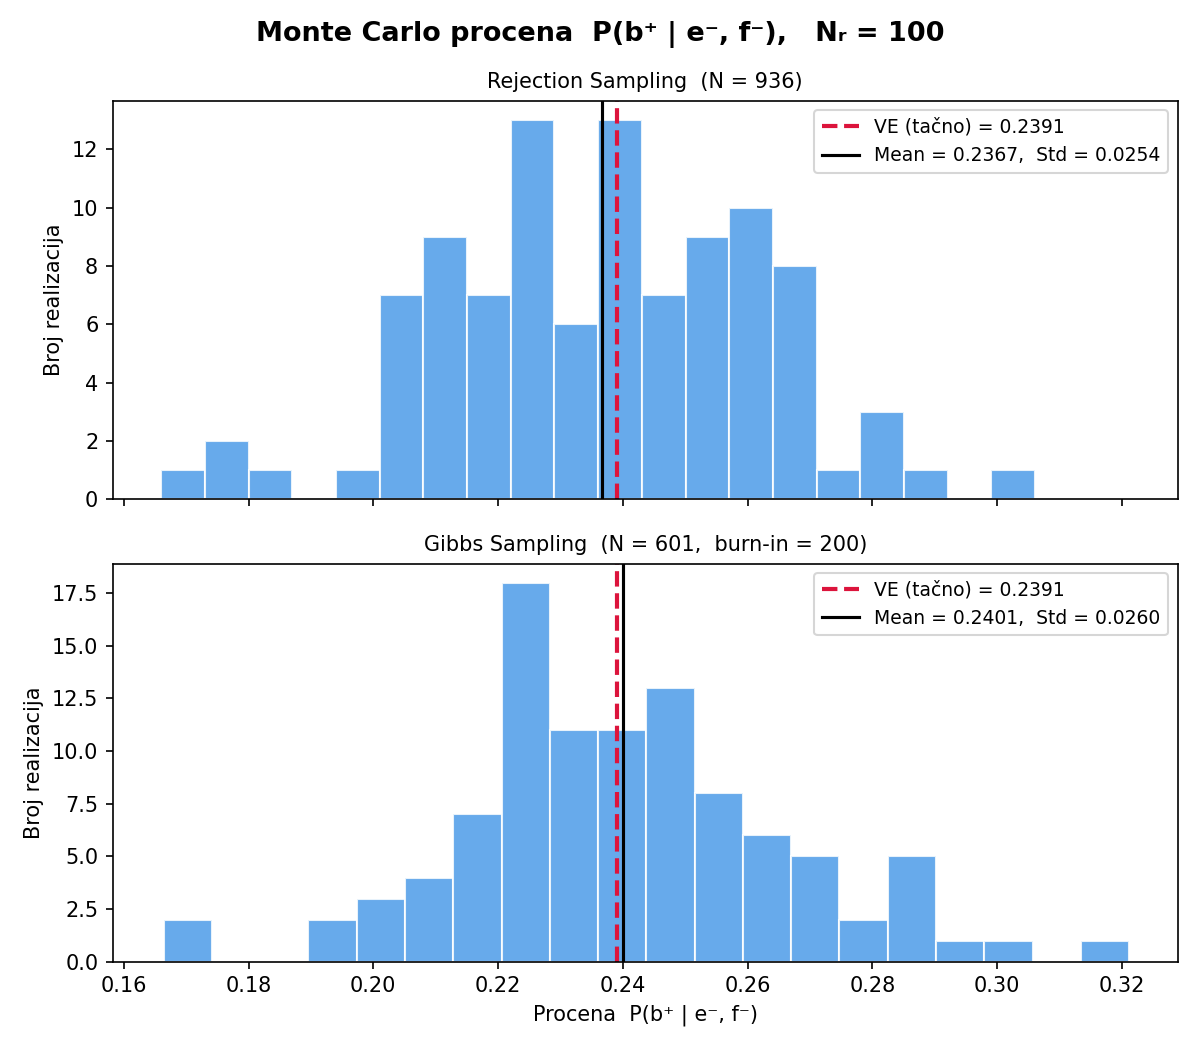
\includegraphics[width=0.82\textwidth]{mc_histograms.png}
  \caption{Histogrami $N_r = 100$ Monte Carlo procena $P(b^+\mid e^-,f^-)$:
           uzorkovanje sa odbacivanjem ($N = 936$) i Gibsovo uzorkovanje
           ($N = 422$, burn-in $= 200$).
           Crvenom isprekidanom linijom označena je tačna vrednost $\approx 0.2391$.}
  \label{fig:mc_hist}
\end{figure}

Obe metode daju procene koje su centrirane oko tačne vrednosti dobijene metodom eliminacije,
sa standardnim devijacijama bliskim ciljnoj vrednosti $\sigma_0 = 0.025$.
Gibsovo uzorkovanje pri tome ne zahteva odbacivanje uzoraka, čime se postiže veća
iskorišćenost generisanih odbiraka. Ipak, korelacija između uzastopnih odbiraka u lancu
smanjuje efektivnu veličinu uzorka ispod nominalne vrednosti $N_\mathrm{Gibbs}$, što
je kompenzovano empirijskom kalibracijom.

\newpage
% =============================================================================
\section{Zadatak 2}

\subsection{Uvod}

Cilj drugog zadatka je praćenje pokretnog objekta čija se pozicija ne može direktno
izmeriti bez šuma. Koristeći čestični filter (ČF) na osnovu zašumljenih merenja
procenjujemo poziciju i brzinu objekta.

Objekat se kreće duž $x$-ose. Njegova pozicija evolucijom u vremenu opisana je
diferentnom jednačinom:
\[
  x[t+1] = x[t] + v[t], \qquad x[0] = 0,
\]
gde je brzina $v[t]$ slučajna promenljiva sa Gaussovom raspodelom:
\[
  v[t] \sim \mathcal{N}\!\left(\mu[t],\,\left(\frac{\mu[t]}{3}\right)^{\!2}\right),
  \qquad \mu[t] = 2^{-t/10}, \quad t = 0,\ldots,49.
\]
Srednja vrednost brzine $\mu[t]$ eksponencijalno opada sa vremenom, što znači da se
objekat postepeno usporava i teži asimptotski nekoj konačnoj poziciji.

Model merenja uzima u obzir mogućnost grubih outlier-a. Merenje $e[t]$ dato je sa:
\[
  e[t] = \theta[t]\cdot x[t] + n[t],
\]
gde je $\theta[t] \sim \mathrm{Bernoulli}(0.9)$, sa verovatnoćom $0.1$ merenje
ne sadrži informaciju o poziciji i sastoji se isključivo od šuma. Šum $n[t]$ prati
Laplaceovu raspodelu nulte sredine čija disperzija raste sa udaljenošću objekta:
\[
  p(n[t]\mid x[t]) = \frac{1}{2\,b(x[t])}\,
  \exp\!\left(-\frac{|n[t]|}{b(x[t])}\right),
  \qquad b(x[t]) = \frac{\sqrt{|x[t]|}}{5}.
\]

Marginalizacijom po $\theta[t]$ dobija se mešavinska verodostojnost:
\[
  p(e[t]\mid x[t]) = 0.9\cdot\mathrm{Lap}\!\left(e[t]-x[t];\,b\right)
                   + 0.1\cdot\mathrm{Lap}\!\left(e[t];\,b\right),
\]
gde $\mathrm{Lap}(z;\,b) = \frac{1}{2b}e^{-|z|/b}$. Prva komponenta odgovara ispravnim
merenjima blizu stvarne pozicije, a druga grubim outlier-ima koji su raspoređeni
oko nule.

% ─────────────────────────────────────────────────────────────────────────────
\subsection{Rezultati}

\subsubsection*{Simulirana trajektorija}

Jedna realizacija trajektorije dobijena je uzorkovanjem brzina prema navedenom modelu
i kumulativnim sabiranjem. Slika~\ref{fig:trajectory} prikazuje vremensku zavisnost
pozicije i brzine za interval $0 \le t < 50$.

\begin{figure}[H]
  \centering
  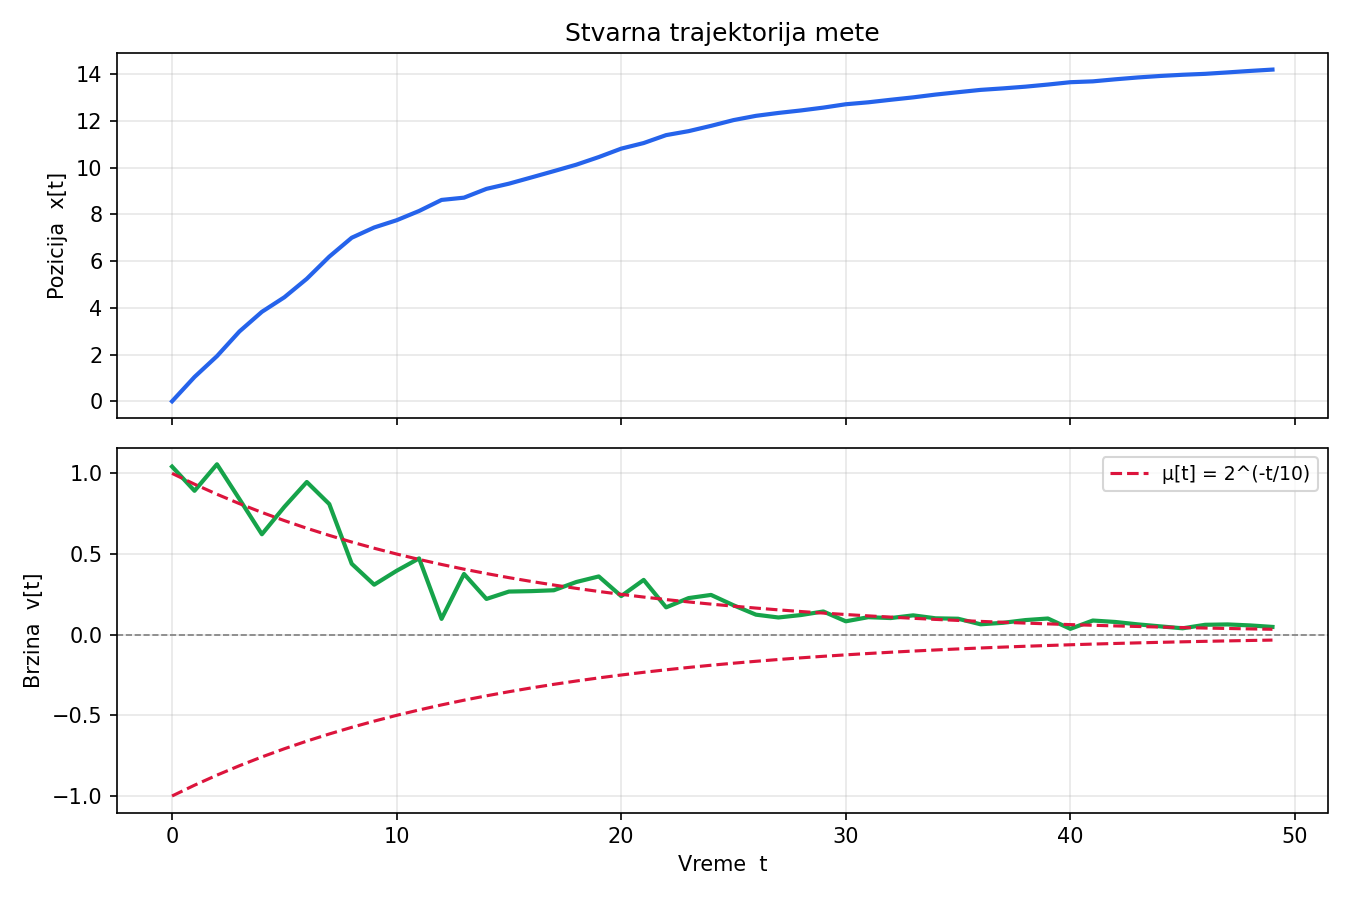
\includegraphics[width=0.82\textwidth]{trajectory.png}
  \caption{Simulirana trajektorija: pozicija $x[t]$ (dole) i brzina $v[t]$ (gore)
           za $t = 0,\ldots,49$. Isprekidana linija prikazuje srednju vrednost brzine
           $\mu[t] = 2^{-t/10}$.}
  \label{fig:trajectory}
\end{figure}

Pozicija monotono raste i teži asimptotskoj vrednosti kako brzina opada.
Brzina fluktuira oko opadajuće srednje vrednosti $\mu[t]$, a njena varijansa
$(\mu[t]/3)^2$ se srazmerno smanjuje, oscilacije su izraženije na početku
i postaju sve slabije kako se objekat usporava.

\subsubsection*{Generisanje opservacija}

Slika~\ref{fig:obs} prikazuje generisane opservacije zajedno sa stvarnom pozicijom.
Merenja kod kojih je $\theta[t] = 1$ (ispravni odbirci) prikazana su zelenom bojom
i nalaze se u blizini stvarne trajektorije, dok su outlier-i ($\theta[t] = 0$)
obeleženi crvenim krstićima i raspoređeni oko nule bez obzira na stvarnu poziciju.

\begin{figure}[H]
  \centering
  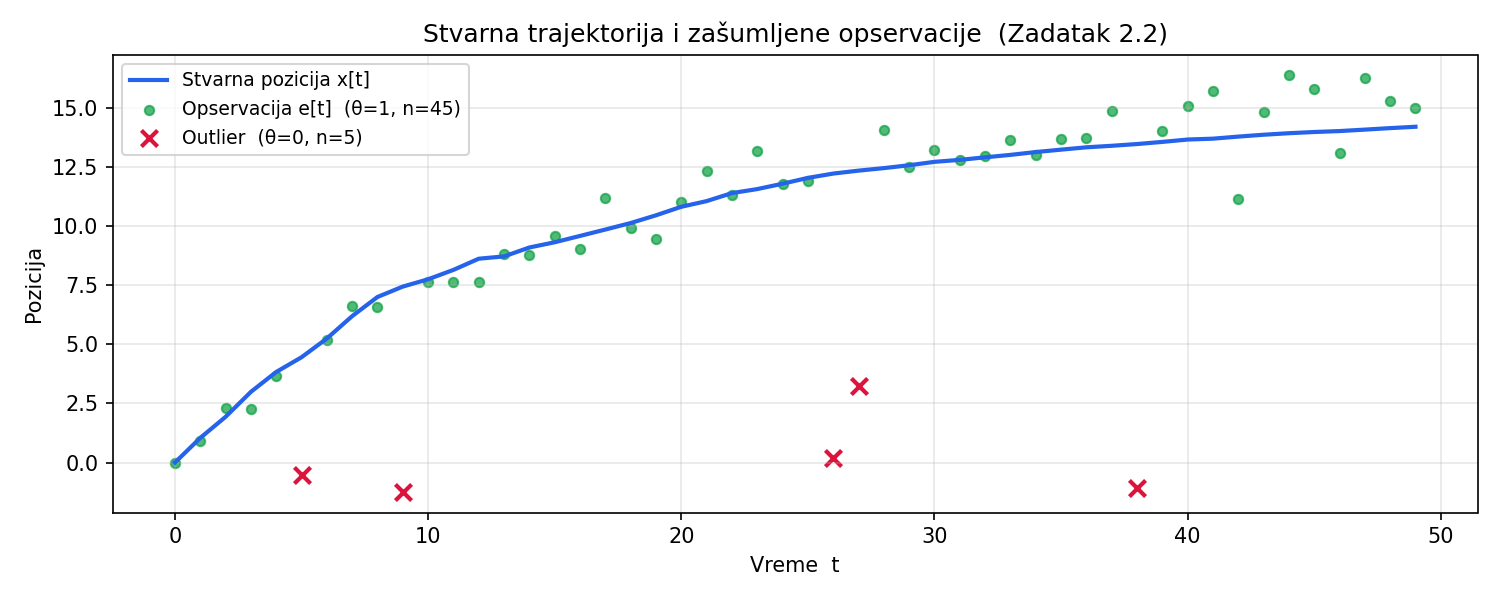
\includegraphics[width=0.82\textwidth]{observations.png}
  \caption{Generisane opservacije $e[t]$: ispravna merenja (zeleni markeri) i
           outlier-i ($\theta[t]=0$, crveni krstići) u odnosu na stvarnu poziciju.}
  \label{fig:obs}
\end{figure}

\subsubsection*{Čestični filter - algoritam i rezultati estimacije}

Čestični filter aproksimira aposteriornu raspodelu stanja $p(x_t \mid e_{0:t})$
skupom $N$ otežinjenih čestica $\{x_t^{(i)}, w_t^{(i)}\}_{i=1}^N$.
Estimacija pozicije dobija se kao ponderisana sredina:
\[
  \hat{x}[t] = \sum_{i=1}^N w_t^{(i)}\,x_t^{(i)}.
\]

Svaka iteracija filtra sastoji se od sledećih koraka:
\begin{enumerate}
  \item \textbf{Ažuriranje i normalizacija težina:}
    log-težine se ažuriraju kao $\log w^{(i)} \mathrel{+}= \log p(e[t]\mid x^{(i)})$,
    zatim se oduzima maksimum i vrši se softmax normalizacija.
    Rad u log-domenu sprečava numeričko potkoračenje koje bi nastalo
    množenjem malih verovatnoća kroz 50 vremenskih koraka.
  \item \textbf{Estimacija:} $\hat{x}[t] = \sum_i w^{(i)} x^{(i)}$.
  \item \textbf{Reuzorkovanje} (po odabranoj strategiji) - opisano u nastavku.
  \item \textbf{Propagacija:} $x^{(i)} \mathrel{+}= v^{(i)}$,
    $v^{(i)} \sim \mathcal{N}(\mu[t],\,(\mu[t]/3)^2)$.
\end{enumerate}

Inicijalno su sve čestice postavljene na $x^{(i)} = 0$, što je konzistentno sa
poznatim početnim uslovom $x[0] = 0$.

Slika~\ref{fig:pf} prikazuje procenjenu i stvarnu poziciju na istom grafiku,
kao i poređenje stvarne i procenjene brzine. Brzina se estimira numeričkim
diferenciranjem pozicije: $\hat{v}[t] = \hat{x}[t+1] - \hat{x}[t]$.

\begin{figure}[H]
  \centering
  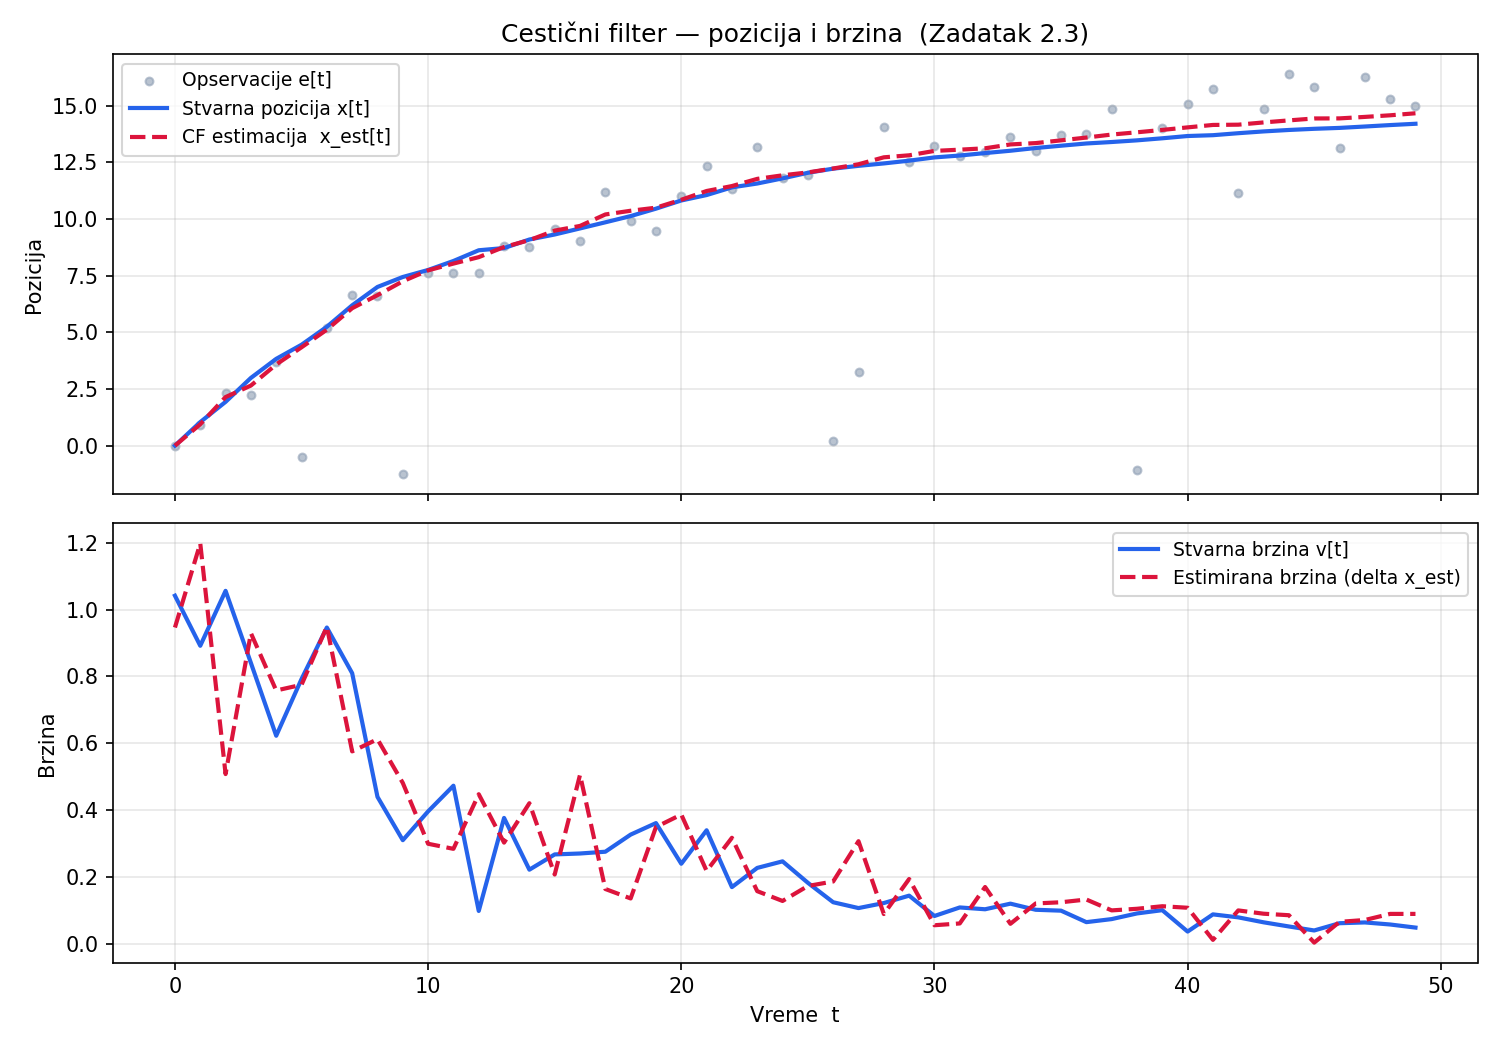
\includegraphics[width=0.82\textwidth]{particle_filter.png}
  \caption{Rezultati čestičnog filtra: estimirana i stvarna pozicija (gore),
           estimirana i stvarna brzina (dole).}
  \label{fig:pf}
\end{figure}

Estimirana pozicija prati stvarnu trajektoriju sa malom greškom, čak i u prisustvu
outlier-a - mešavinska verodostojnost penalizuje čestice daleko od stvarne pozicije
znatno manje agresivno nego čist Gaussov model, pa outlier-i ne remete procenu.
Estimirana brzina dobro reprodukuje opadajući trend, ali pokazuje veće fluktuacije
nego stvarna brzina. To je očekivano: ČF direktno procenjuje poziciju, a brzina
dobijena numeričkim diferenciranjem akumulira greške iz dva uzastopna vremenskog koraka.

\subsubsection*{Vizuelizacija čestica}

Slika~\ref{fig:particles} prikazuje raspodelu čestica u odabranim vremenskim trenucima,
neposredno pre eventualnog reuzorkovanja. Veličina markera proporcionalna je težini
čestice, a boja odražava isti podatak na kontinuiranoj skali.

\begin{figure}[H]
  \centering
  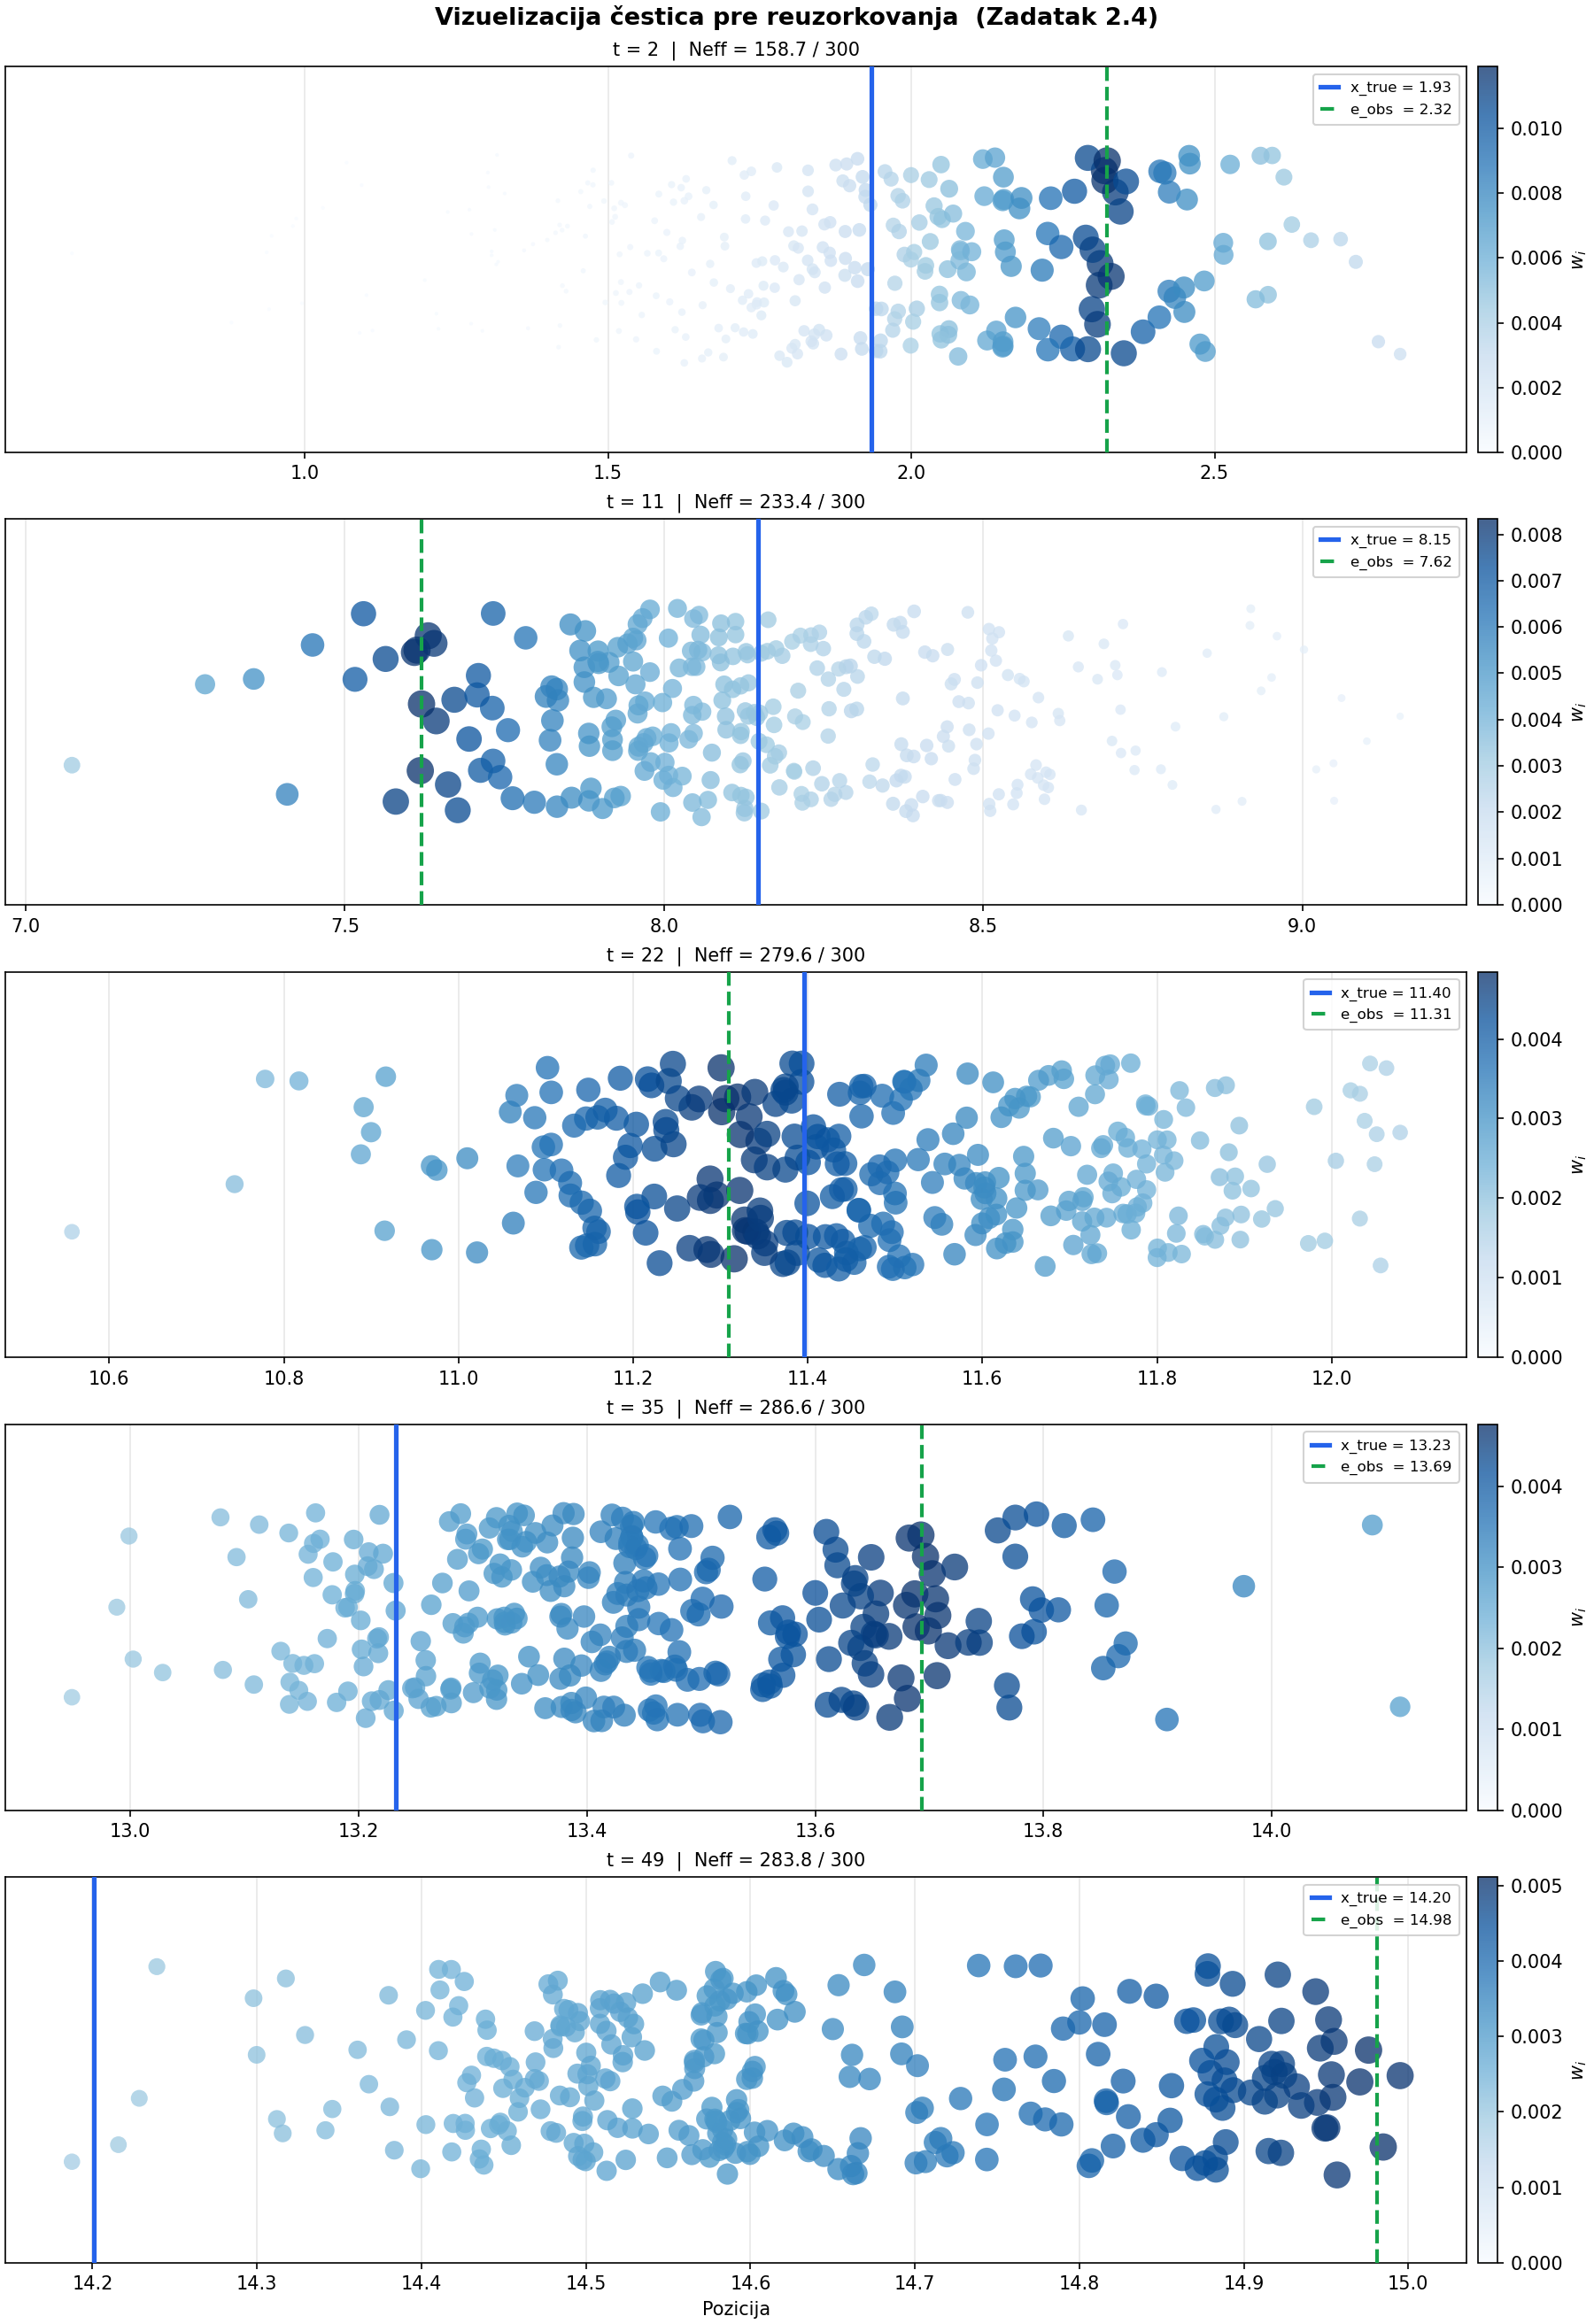
\includegraphics[width=\textwidth]{particles_viz.png}
  \caption{Raspodela čestica (pre reuzorkovanja) u odabranim trenucima.
           Vertikalna plava linija označava stvarnu poziciju, zelena isprekidana
           linija označava izmerenu vrednost.}
  \label{fig:particles}
\end{figure}

Na ranim vremenskim koracima čestice su razmaknute i težine su relativno ujednačene
(velika efektivna veličina $N_\mathrm{eff}$). Kako vreme prolazi, težine se
koncentruju na uski skup čestica bliskih stvarnoj poziciji, a $N_\mathrm{eff}$
opada. Outlier-i ne pomeraju masu čestica ka nuli zbog toga što verodostojnost
smanjuje težine outlier pozicija, a ne eliminiše ih odmah.

\subsubsection*{Uticaj strategije reuzorkovanja}

Degeneracija težina fundamentalni je problem čestičnih filtara: kroz iteracije,
sve veća masa verovatnoće koncentruje se na manjem broju čestica, dok ostatak
praktično ne doprinosi estimaciji. Reuzorkovanje je mehanizam kojim se eliminišu
čestice male težine i multipliciraju one sa velikom težinom, čime se obnavlja
raznolikost skupa čestica.

\paragraph{Bez reuzorkovanja.}
Bez ikakvog reuzorkovanja, log-težine se kumulativno sabiraju kroz sve iteracije
i neizbežno dolazi do degeneracije - efektivna veličina uzorka:
\[
  N_\mathrm{eff} = \frac{1}{\sum_{i=1}^N (w^{(i)})^2}
\]
opada ka 1, što znači da jedna čestica nosi praktično svu masu.
Estimacija tada postaje loša aproksimacija prave aposteriorne raspodele,
a RMSE pozicije je najveći od sve tri strategije.

\paragraph{Reuzorkovanje u svakoj iteraciji.}
Multinomijalno reuzorkovanje u svakom vremenskom koraku sprečava degeneraciju:
čestice se biraju sa ponavljanjem proporcionalno njihovim težinama, a težine se
resetuju na $1/N$. Ovo poboljšava estimaciju u poređenju sa odsustvom reuzorkovanja.
Međutim, česta primena unosi i novi problem - osiromašenje čestica (\textit{sample
impoverishment}): ponavljanim uzorkovanjem raznolikost čestica se smanjuje jer
više kopija iste čestice propagira kroz isti šum. Kada je $N_\mathrm{eff}$ još
uvek velik (težine su relativno ujednačene), reuzorkovanje je nepotrebno i
uvodi suvišnu statističku grešku.

\paragraph{Adaptivno reuzorkovanje.}
Kompromis između prethodne dve strategije: reuzorkovanje se vrši samo kada
efektivna veličina uzorka padne ispod praga $N_\mathrm{eff} < N/2$.
Na taj način se interveniše jedino kad je degeneracija zaista problem,
čuvajući raznolikost čestica dok su težine dobro distribuirane.
Ova strategija daje najmanji RMSE i najmanju varijansu greške od sve tri.

\subsubsection*{Monte Carlo analiza - poređenje RMSE ($N_r = 500$)}

Kroz 500 nezavisnih Monte Carlo simulacija, za svaku strategiju reuzorkovanja
izračunat je koren srednje kvadratne greške pozicije:
\[
  \mathrm{RMSE} = \sqrt{\frac{1}{T}\sum_{t=0}^{T-1}(\hat{x}[t] - x[t])^2}.
\]
U svakoj simulaciji koriste se isti $x_\mathrm{true}$ i $e_\mathrm{obs}$, a razlikuje
se samo generator slučajnih brojeva čestičnog filtra, čime se osigurava pošteno poređenje.
Broj čestica je $N = 100$. Raspodele RMSE za sve tri strategije prikazane su na slici~\ref{fig:rmse}.

\begin{figure}[H]
  \centering
  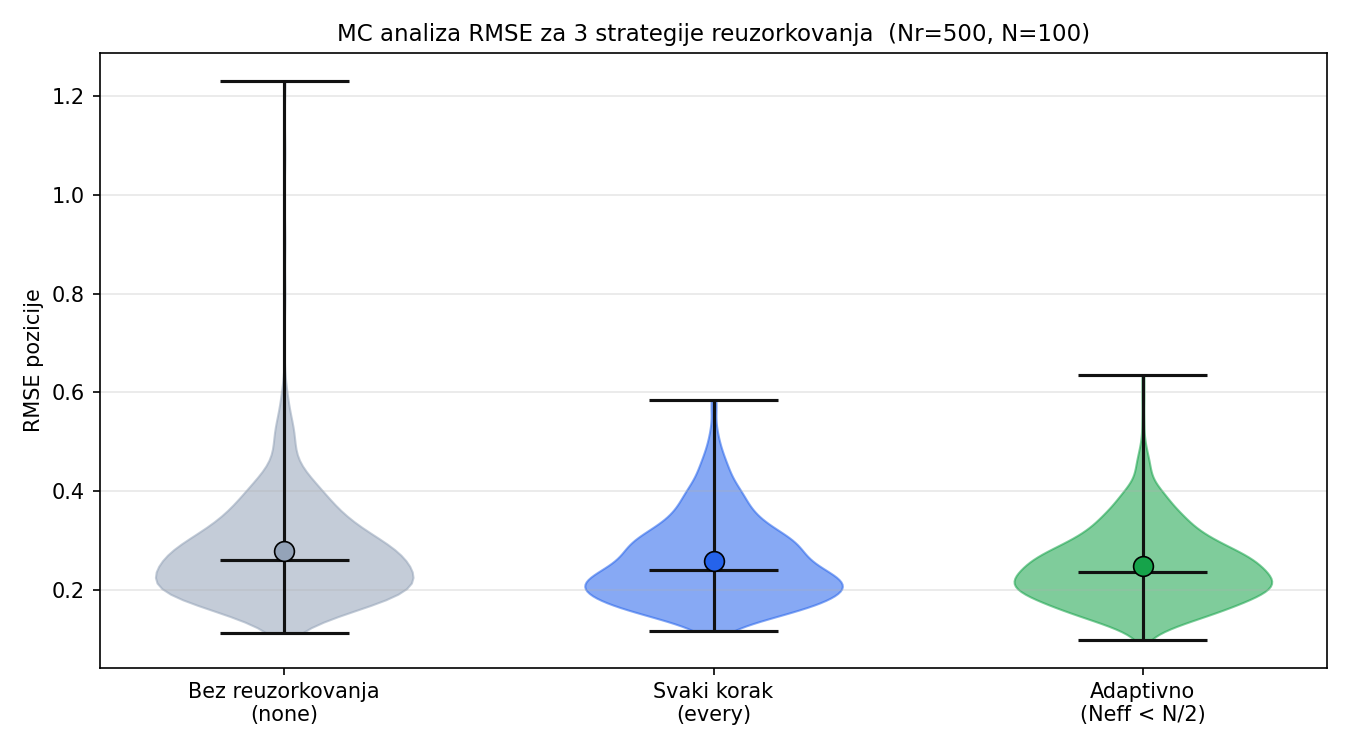
\includegraphics[width=0.82\textwidth]{mc_rmse.png}
  \caption{Raspodela RMSE pozicije za tri strategije reuzorkovanja kroz 500 Monte Carlo
           simulacija ($N = 100$ čestica). Violinski dijagrami prikazuju celu empirijsku
           raspodelu, uključujući outlier-e.}
  \label{fig:rmse}
\end{figure}

Rezultati potvrđuju teorijska očekivanja: adaptivno reuzorkovanje postiže i najmanji
srednji RMSE i najmanju varijansu, dok odsustvo reuzorkovanja daje najgore rezultate.
Strategija reuzorkovanja u svakoj iteraciji nalazi se između, što ukazuje da prečesto
reuzorkovanje, iako sprečava degeneraciju, uvodi osiromašenje čestica koje delimično
poništava dobit. Sve tri strategije dele sličnu donju granicu RMSE, što odražava
inherentnu nesigurnost zadatka - informacioni sadržaj merenja ograničava maksimalnu
tačnost bez obzira na strategiju.

\end{document}

